\documentclass{article}
\title{Software Development M \\
LoRa - Network Capacity Analysis}
\author{
Martin Fleischer \\
\texttt{martin.fleischer@tu-berlin.de} \\
\small Prof. Oreste Andrisano \\
\small \texttt{oreste.andrisano@unibo.it} \\
\small Flavio Zabini \\
\small \texttt{flavio.zabini2@unibo.it}
}
\date{\today}

\usepackage{listings}
\usepackage{hyperref}
\hypersetup{colorlinks,urlcolor=blue}
\usepackage[title]{appendix}
\usepackage{graphicx}

\graphicspath{{../figures}}

\begin{document}
\maketitle
\tableofcontents

\section{Introduction}
This section introduces motivation and goals of the project activity performed
in scope of the module Software Development M of the degree program
Telecommunications Engineering at the Universit\`{a} di Bologna.

\subsection{Description}
The project goal defined by the authors of this report is the implementation of
a simulator, able to reproduce plots similar to the ones reported in
\cite{augustin2016study, adelantado2017understanding}. Among other
observations, both papers present plots that help to understand the capacity
limitations of LoRaWANs. LoRaWANs are collision prone and present contention
similar to pure ALOHA access, except LoRaWAN allows different packet sizes. In
addition, the industrial, scientific and medical (ISM) bands, in which LoRaWAN
operates, require fair use policies i.e. duty-cycled band access, that need to
be accounted for in performance evaluations. The physical layer parameters of
the LoRa modulation influence the performance of the network and different
settings require proper analysis. Understanding the limits reveals crucial
insights for finding appropriate dimensioning and device configuration of a
LoRaWAN.

\section{LoRa and LoRaWAN}
This chapter summarizes LoRa and LoRaWAN briefly and defines the essential
parameters required for the implementation of our LoRaWAN channel simulations.

\subsection{Overview}
The LoRa protocol stack can be categorized as a set of protocols providing
specifications for operating a LPWAN (Low Power Wide Area Network). LPWAN
protocols offer solutions for running networks of low energy devices, e.g.
sensors over long communication distances, typically in the range of several
kilometers. Besides some competitors LoRa is one of the emerging protocol
stacks foreseen to provide solutions for future IoT (Internet of the Things)
networks connecting billions of devices.\\

There is a crucial differentiation between LoRa (Long Range) and LoRaWAN (Long
Range Wide Area Network), which are often fleetly referred to as LoRa. More
precisely, LoRa and LoRaWAN refer to the physical and the MAC layer of the LoRa
protocol stack.

The former specifies a proprietary PHY layer technology developed by Semtech.
LoRa is based on Chirp Spread Spectrum modulation and operates in the ISM
bands. The physical layer aims at high robustness against interference and high
immunity against the Doppler Effect \cite{augustin2016study,
loramodulationbasics}. LoRa has no open specification, however there are
projects and research activities that have reverse engineered and analyzed
parts of the LoRa PHY layer technology \cite{knight2016decoding,
sikkendecodinglora}.

LoRaWAN (Long Range Wide Area Network) is the MAC layer protocol of the
protocol stack. The protocol is specified by the LoRa Alliance that builds on
LoRa modulation or FSK (Frequency Shift Keying) \cite{lorawanspec}. The network
architecture of LoRaWAN specifies a star-of-star topology of
\textbf{end-devices}, \textbf{gateways}, and a central \textbf{network server}
in the backend. More recent publications separate the functionality of the
backend and define interfaces between the components \cite{lorawanbackend}.
Although, the backend functionality can be separated in different components we
refer to a central network server with collocated backend functionalities in
this document. End-devices are typically sensors or actuators with limited data
rate requirements, short messages and low traffic intensity, e.g. few messages
per day. There are three different end-device classes (Class A, B, and C) with
different scheduling schemes for downlink communication. Gateways are message
relays between end-devices and the network server. While end-devices
communicate with the gateways over LoRa or FSK, the backhaul connectivity
between gateways and the network server is based on IP and offers a much higher
capacity, e.g. Ethernet or 3G \cite{lorawanspec, augustin2016study}.

\subsection{LoRa parameters}
An understanding of the operational parameters introduced in this section is
critical for the development of our LoRaWAN channel simulator. Adjustment of
these parameters allows tuning the trade offs between throughput, communication
range and reliability.\\

The throughput of every radio communication obviously depend on the signal
\textbf{Bandwidth} (BW). The ISM bands regulations offer several channels with
different sizes. Typical sizes of the LoRaWAN channels in Europe are 125, 250
and 500 kHz.  The LoRa modulation spreads the data stream to one chip per
second per Herz. Therefore, an increase of the BW will accelerate the data
transmission, but must be traded against a reduced receiver sensitivity by the
introduction of additional noise. Vice versa, decreasing the bandwidth results
in higher receiver sensitivity, though increases the \textbf{Time on Air}
\cite{loramodulationbasics, loramodem}.\\

LoRa is a Direct Sequence Spread Spectrum (DSSS) technology and it's
\textbf{Spreading Factor} (SF) determines the chip composition per symbol.
Since LoRa modulation uses $2^{SF}$ chips per symbol, the chipping used by LoRa
relates bit rate and chip rate by \cite{loramodulationbasics}: 

$$R_{c} = 2^{SF} R_{b}$$

LoRa offers SFs between 7 and 12. The codes used for the different SFs are
orthogonal to each other, i.e. signals with different spreading factors can be
transmitted simultaneously. Therefore, the pair of operating frequency and
spreading factor composes a logical channel \cite{augustin2016study}. The
symbol time of LoRa is given by the formula \cite{loramodulationbasics}:

$$T_{s} = \frac{2^{SF}}{BW}\,s$$

Consequently, higher spreading factors increase the symbol duration leading to
an increased Time on Air, but also increase the receiver sensitivity.
Therefore, higher SFs can increase the transmission range.\\

Finally, the \textbf{Code Rate} defines the redundancy bits used by LoRa's
Forward Error Correction (FEC) mechanism. Possible values for the CR are in
$[1,2,3,4]$ corresponding to the coding rates of $[\frac{4}{5}, \frac{4}{6},
\frac{4}{7}, \frac{4}{8}]$ resulting in the formula
\cite{loramodulationbasics}:

$$\textrm{Rate Code} = \frac{4}{4+CR}$$

Decreasing the Rate Code, respectively increasing the CR result in lower Packet
Error Rates (PER), but also increases the Time on Air \cite{augustin2016study,
loramodulationbasics}.

\subsection{Regulations}

LoRa devices operate in the ISM bands. The LoRa alliance summarizes regulatory
parameters in \cite{lorawanregparams}. For Europe the ISM bands EU 863-870MHz
and the EU 433MHz are available.

Paradoxically, LoRa transceivers fall in the category of Short Range Devices
(SRD). The license free operating bands for SRDs are defined by the ERC REC
70-03 \cite{recommendation200970}. Devices have to meet the regulatory
requirements of ETSI EN 300 220-2 \cite{etsisrd2018}. ETSI allows devices to
operate in the ISM bands either by implementing a Listen Before Talk (LBT)
mechanism or by limiting operation to duty cycles, which are dependent on the
chosen sub-band. Current LoRaWAN standards operate in the ladder, duty-cylcled
mode, exclusively \cite{lorawanregparams}. A slightly outdated document by
Semtech summarizes the regulations and the corresponding duty cycles for the
LoRa Modem design \cite{loraetsicompliance}.

\subsection{Time on air Calculation}
For the detection of colliding packets, it is necessary to compute the duration
of a packet, respectively it's Time on Air. The LoRa modulation spreads its
symbols over the whole spectrum with bandwidth in Hertz equal to the chip rate,
e.g. a programmed bandwidth of 125kHz implicates a chip rate of 125 kcps.

A packet consists of a Preamble, followed by a header encoded with a code rate
of $\frac{4}{8}$ and protected by a CRC. The Payload and it's CRC are encoded
by the programmed code rate. Figure \ref{fig:packetformat} is taken from
\cite{loramodem} to visualize the packet format.

\begin{figure}
    \centering
    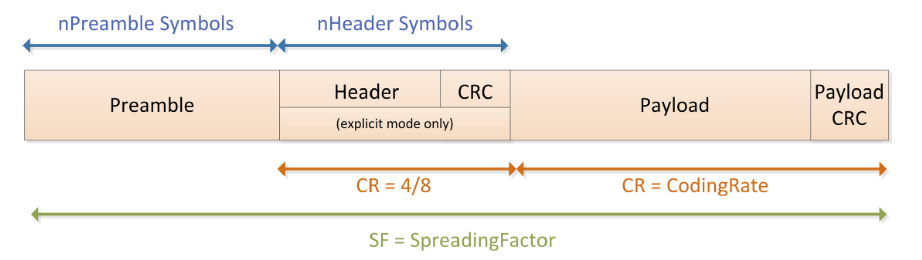
\includegraphics[width=0.8\textwidth]{./figures/packet_format}
    \caption{LoRa PHY layer packet format \cite{loramodem}}
    \label{fig:packetformat}
\end{figure}

The preamble duration depends on the number of preamble symbols configured and
can be calculated by following formula:

$$T_{preamble} = ( n_{preamble} + 4.25 ) \, T_{sym}$$

The number of symbols of the packet payload is calculated by \cite{loramodem}:

$$ \textrm{payloadSymbNb} = 8 + max \left( ceil \left( \frac{ 8PL - 4SF + 28 + 16 - 20H }{ 4 \left( SF - 2DE \right) } \right) \left( CR + 4 \right) , 0 \right) $$

Where:
\begin{itemize}
        \item PL: Payload bytes
        \item SF: Spreading Factor
        \item H: Header; 0 = enabled, 1 = no header
        \item DE: Low Data Rate Optimization; 1 = enabled , 0 = disabled.
        \item CR: Coding rate
\end{itemize}
\vspace*{\baselineskip}

The header option H can be set to 1 to indicate fixed length packets. In this
case the header can be omitted to reduce the payload length. The Low Data Rate
Optimization can help to make the communication more robust to frequency
variations \cite{loramodem}. This option is not accurately documented in the
manuals and guides provided by Semtech, but the formula for the payload symbol
calculation reveals that decreases the number of transmitted bits per symbol by
a factor of 2 \cite{augustin2016study}.

Finally, the total duration of the packet can be calculated by summing up the
preamble and the payload duration:

$$T_{packet} = T_{preamble} + T_{payload}$$

All formulas of this section have been adopted from \cite{loramodem}. Also
\cite{augustin2016study} describes the physical parameters of the LoRa
modulation and derives a slightly different formula for the computation of the
payload symbol number. Semtech provides a LoRa Calculator that helps to compute
the Time on Air. In addition, a spreadsheet developed in The Things Network
(TTN) community is discussed in the forum in \cite{loraspreadsheet} and can be
accessed through a web link.

\section{LoRaWAN Collision Rate simulation}\label{sec:simulator}
Our collision rate simulation requires three separate steps. At first, packets
generated by each device are simulated. In the second step, the simulator
writes the generated packets in a single table and searches for packet
collisions. At last, the resulting collision rate is calculated per device
number. A plot visualizes the device number at the abscissa against the
collision rate at the ordinate.

In the first step the simulator generates packets for a given simulation
duration. The physical layer parameters can be configured:

\begin{itemize}
    \item BW: Bandwidth
    \item SF: Spreading Factor
    \item CR: Code Rate
    \item DE: Data Rate Optimization
\end{itemize}
\vspace*{\baselineskip}

Furthermore, the distribution for the packet arrival can be configured. For our
simulations reported in this paper a Poisson distribution was chosen. The
arrival rate $\lambda$ of the Poisson process can be defined and determines the
mean time difference between two packets in milliseconds. The minimum and
maximum packet size in bytes (packetDistLower, packetDistUpper), the duty cycle
limitation (dc), preamble length (nPreamble), and disabling of the header (h)
are set. Finally, the number of devices (numDevices) operating in the channel
can be configured for the simulation. 

The simulator generates packets for each device, corresponding to numDevices. A
random packet length uniformly distributed between packetDistLower and
packetDistUpper is randomly assigned for each packet. The arrival time of a
packet is Poisson distributed, but has to respect the duty cycle. The algorithm
for meeting the regulatory duty cycle restriction was implemented as specified
by the LoRaWAN Specification 1.0. A backoff time (Toff) is calculated by the
formula given in the specification:

$$ Toff = \frac{TimeOnAir}{DutyCycle} - TimeOnAir$$

After sending a packet, devices wait at least for Toff, before they send the
next packet. If the arrival time of the next packet generated by the Poisson
process has a silent period lower than Toff, the start time of the next packet
is set to $\textrm{previous arrival time} + Toff$. The latest LoRaWAN
specification leaves the implementation of the algorithm guaranteeing the
compliance to the duty cycle restriction open to the manufacturer.

The result of the device simulations are text files for each device, containing
packets represented by Arrival Time, End Time, Packet Length, and Time On Air
in CSV format.

The second step of the collision rate simulation finds colliding packets,
calculates. All packets generated by the devices are read into a single table,
the collision table. The packets are sorted by arrival date. Collisions are
calculated by determining if the duration between a packet arrival and the
packet end overlaps with the duration of another packet. The following pseudo
code shows the condition for a packet collision:

\begin{lstlisting}
(other_end >= arrival & other_arrival <= end) |
(end >= other_arrival & arrival <= other_end)
\end{lstlisting}

The results of the collision calculation, the collision table, is written to a
single CSV file. The output file contains all packets, sent by all devices, the
packets are ordered by arrival date. Packets in the CSV file are represented by
following values.

\begin{itemize}
        \item Id: Packet identifier, packets with earlier arrival time have a
                lower id starting from 1. If the arrival time overlaps with
                another packet, the packet sent by the lower device id receives
                the lower id.

        \item Arrival: Date time of the packet arrival. 

        \item End: End time of the arrival, calculated as $Arrival + TimeOnAir$

        \item PacketLength: Length of the packet in bytes.

        \item TimeOnAir: Duration of the packet.

        \item Device: Identifier of the device, numbered from 1 to the maximum
                device number parameter of the simulation.

        \item Collisions: A space separated list of Ids of colliding packets.
\end{itemize}
\vspace*{\baselineskip}

In the final step the collision table is read to calculate the collision rate,
i.e. the number of collided packets divided by the total packets sent.  No
capture effect is considered, i.e. all packets with collisions are considered
as lost. The simulator calculates the collision rate for a linear decreasing
number of devices up to numDevices. The device number on the abscissa shows how
many devices have been considered for the collision rate calculation. For each
value the first x devices are chosen. The ordinate shows the corresponding
collision rate.

\subsection{Analysis of the reference plot}
To verify the results of our simulator, we decided to take a reference plot
from Augustin et al. and compare it with our simulations
\cite{augustin2016study}. This plot is shown in Figure
\ref{fig:collissionrateaugustin} and was chosen, because the simulation
parameters have been reported rigorously. The graph of Augustin et al. shows
the collision rate and the channel utilization simulated for a single logical
LoRaWAN channel. Table \ref{table:augustinparams} summarizes the parameters of
their simulation.

\begin{figure}
    \centering
    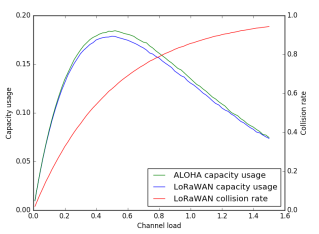
\includegraphics[width=0.5\textwidth]{./figures/a_study_of_lora_collision_rate}
    \caption{Collision Rate plot from \cite{augustin2016study}}
    \label{fig:collissionrateaugustin}
\end{figure}

\begin{table}
\begin{tabular}{ | l | l | l | l | l | l | l | l | }
\hline
        BW      & SF & CR & DE & payload length  & DC   & nPreamble & H \\
\hline
        125 MHz & 7  & 5  & 0  & 1 - 51 bytes    & 1\%  &   6       & 1 \\
\hline
\end{tabular}
\caption{Simulation parameters reported by Augustin et al.
        \cite{augustin2016study}}
\label{table:augustinparams}
\end{table}

The reported rate code of $\frac{5}{4}$ is probably a mistake, since it is not
a feasible value. We suppose a rate code of $\frac{4}{5}$, with a CR of 5 has
been selected. Different payload size implicate that headers are enabled, even
if it is not explicitly stated.

Instead of a fixed simulation duration Augustin et al. report that
five-hundred-thousand packet have been generated per data point. The Collision
rate can be read from the right side of the ordinate. The Channel load on the
abscissa, is evaluated by the number of devices accessing the channel over the
simulation period. That means, in a perfectly synchronized network 100 devices
can achieve a channel load of 1 for a duty cycle restriction of 1\%. Following
formula computes the ideal Channel Load for a given device number: 

$$ \textrm{Channel load} = \textrm{Number of devices} \cdot DC$$

The Capacity Usage on the left side of the plot is the data successfully
transmitted during the simulation divided by the theoretical maximum throughput
of a LoRa channel: 

$$\textrm{Capacity Usage} = \textrm{Channel Capacity} \cdot \textrm{simulation
duration}$$

The evaluation of the channel capacity follows the calculations of the network
planing example in \cite{loramodulationbasics}. Our plots do not show the
capacity usage, but the data of our collision table contains all required
information for its calculation. The channel capacity can be calculated by
following formulas:

$$\textrm{Channel Capacity} = \frac{\textrm{successfully received
data}}{\textrm{maximum theortical capacity}}$$

The packet sizes in \cite{augustin2016study} were uniformly distributed between
1 and 51 bytes. In our simulations we added MAC payload of 13 bytes to the
distribution, which is the minimum MAC Payload of a LoRaWAN packet according to
Augustin et al. \cite{augustin2016study}. The consideration of the minimum MAC
payload was not explicitly stated for the Collision Rate simulation in
\cite{augustin2016study}.

Augustin et al. chose a Poisson distributed arrival process for the packets.
The arrival rate of the simulation was not reported. For our first experiment
we chose an arrival rate close to the duty cycle limitations. The extraordinary
value of 7138 derives from following calculations.

Average Time on Air for payload length between 14 and 51 bytes:
$$\overline{TimeOnAir} = \frac{1}{38} \sum_{n=14}^{51} TimeOnAir_{n} = 71.370\, ms$$

Maximum airtime per hour for a duty cycle of 1\%:
$$MaxAirtime/h = 3600*1000*0.01 = 36000\, ms$$

Average packets per hour:
$$\overline{packets/h} = \frac{MaxAirtime/h}{\overline{TimeOnAir}} = 504.413\, packets$$

Arrival rate:
$$\lambda = \frac{3600000\, ms}{\overline{packets/hour}} = 7137.010526$$

\subsection{Results}
The same parameters as reported in \cite{augustin2016study} have been selected
for our simulation. The tables \ref{table:phy_params} and
\ref{table:sim_params} summarize the simulation parameters.

\begin{table}
\begin{tabular}{ | l | l | l | l | l | l | l | l | }
\hline
        BW      & SF & CR & DE & PacketLength  & DC   & nPreamble & H \\ \hline
        125 MHz & 7  & 5  & 0  & 14 - 51 bytes & 1\% & 6         & 1 \\
\hline
\end{tabular}
\caption{PHY parameters}
\label{table:phy_params}
\end{table}

\begin{table}
\begin{tabular}{ | l | l | l | l | }
\hline
        Simulation Duration & Distribution & lambda & Number of Devices \\ \hline
        3h                  & Poisson      & 7138   & 160 \\
\hline
\end{tabular}
\caption{Simulation parameters}
\label{table:sim_params}
\end{table}

Figure \ref{fig:collissionratecomparison} shows our first experiment. The
collision rate computed with our simulator in blue in comparison with the
collision rate reported by Augustin et al. \cite{augustin2016study} in red. The
plots have been overlaid with graphic tools, since the data is to our best
knowledge not publicly available. Therefore, the red curve from the reference
plot is not exact. However, the tendency of a similar collision rate can be
seen. The steps in the curve of our collision rate provide evidence that we do
not collect enough data and we need to increase the simulation duration,
nevertheless the tendency is recognizable.\\

\begin{figure}[h]
    \centering
    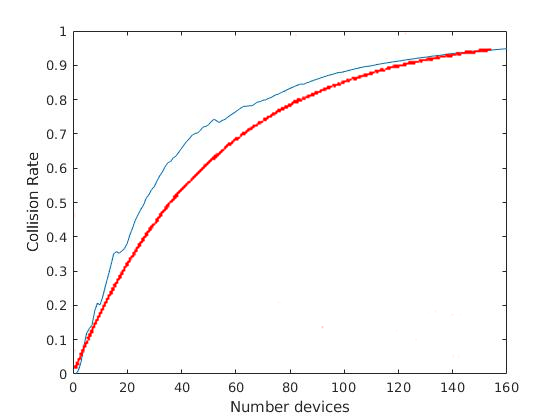
\includegraphics[width=0.8\textwidth]{./figures/collision_rate_compare_lambda7138}
    \caption{Collision Rate comparison}
    \label{fig:collissionratecomparison}
\end{figure}

Altogether, the number of collisions in our plots clearly tends to be higher.
We have two major explanations for that. Firstly, Augustin et al. have not
precisely documented the packet arrival process. We have chosen an arrival rate
close to maximum duty cycle. A more relaxed choice of the arrival rate reduces
the collisions. Plotting the channel usage as well, could have helped finding
an analog arrival rate, since an arrival process far from the duty cycle also
reduces the channel usage.

In addition, we have stated before, Augustin et al. have not explicitly
reported that the minimum MAC payload of 13 bytes was considered in their plot.
Another experiment reported in the paper explicitly states this consideration.
A smaller average payload size also explains smaller number of collisions.

Furthermore, we have another minor consideration about the collision behavior
in the LoRaWAN network. The algorithm to comply with ETSI's duty cycle
restrictions was fixed in revision 1.0 of the LoRaWAN specification. This
restriction was dropped in revision 1.1 \cite{lorawanspec}.  The algorithm used
by Augustin et al. was not reported. A neat choice of the implementation of the
duty cycle protection could be also useful for reduction of collisions. Such
solutions are certainly application respectively traffic specific and can be an
interesting research opportunity in our opinion.\\

To verify our assumptions we have conducted experiments with different
parameter settings. Firstly, we ran the simulation with slightly increased
arrival rates to relax the contention. Then, we have also removed the minimum
MAC payload size of 13 bytes resulting in a uniform payload size distribution
in the interval [1,51] bytes. Figure \ref{fig:collissionratecomparisonfinal}
shows in blue our first experiment reported in the beginning of this section.
The green curves show simulation results with relaxed arrival rates $\lambda$
of 8000 (straight) respectively 9000 ms (dashed) between packet arrivals. The
curve in magenta shows the curve with an arrival rate of 7138, equal to our
first experiment, but with a uniform payload length distribution in the
interval between [1,51] bytes. The results confirm our assumptions, either
relaxing the arrival rate or reducing the packet length in average brings us
closer to the curve reported by Augustin et al. which has been graphically
overlaid in the red curve. Especially, the curve with reduced minimum payload
length looks very close to the curves in \cite{augustin2016study}. As we have
already stated, both increasing the inter-arrival time and reducing the payload
length in average results in lower Channel Load. The Channel Load should be
also investigated to verify the comparability. 

\begin{figure}[h]
    \centering
    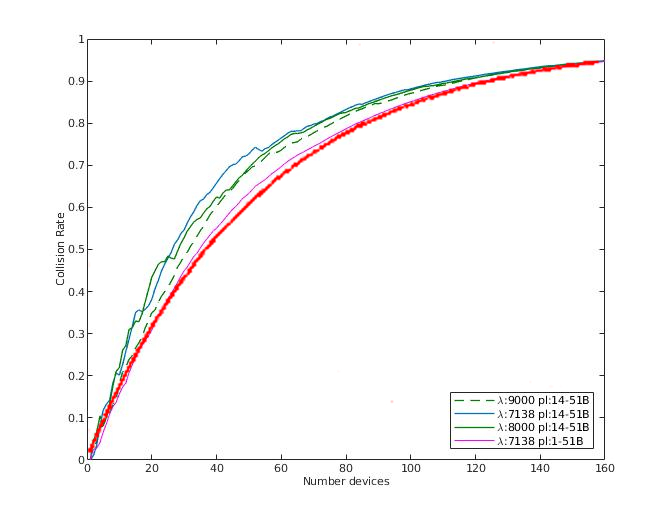
\includegraphics[width=1\textwidth]{./figures/collision_rate_compare_final}
    \caption{Collision Rate comparison with different parameters}
    \label{fig:collissionratecomparisonfinal}
\end{figure}

\section{Conclusion}
To a greater extend, we were able to verify the results of the collision rate
simulations in a single logical LoRaWAN channel reported by Augustin et al.
\cite{augustin2016study}.

For a more precise comparability with the experiment reported in
\cite{augustin2016study} and to find the appropriate simulation parameters we
should also compare the Capacity Usage. Besides, there exists plenty of other
research, analyzing performance of LoRaWANs. Especially, analytical approaches,
e.g. Markov-Chain based performance evaluation, could increase the verification
of the simulation results. Such approaches have been reported in
\cite{sorensen2017analysis, delobel2017analysis, ferre2017collision}.
Extending the analyses, e.g. to other device types and to the confirmed
messages, would improve the utility of our simulator greatly.

Augustin et al. conclude, that the channel load in the network significantly
influences the performance of the network. However, the simulation of a single
channel does not reflect the capacity of a LoRaWAN. On one hand, the LoRa
protocol stack is not designed for devices sending packets at high transmission
frequency. Rather, LoRaWAN has been designed with sensors and actuators in mind
consuming very low amounts of energy. The energy requirements of such devices
prohibit high frequent traffic as investigated in the presented simulations. On
the other hand, LoRaWAN prescribes the usage of several default channels, e.g.
for the EU863-870 ISM Band at least the channels 868.10, 868.30 and 868.50 have
to be supported for device access in a pseudo-random manner \cite{lorawanspec,
lorawanregparams}. Moreover, the orthogonality of the SF logically separates
the channels even further, reducing the contention in a single logical channel.
In conclusion, the simulations still shows that network operators have to
analyse the traffic requirements of the network and choose the operating
parameters of LoRaWAN carefully.

\newpage
\begin{appendices}

        \section{Collision Rate Simulator - User manual}
        This section briefly shows how to run the simulation software described
        in the report. The operation mode of the simulator is described in
        \ref{sec:simulator}. Figure \ref{fig:simulation} visualizes the steps
        we described in the report.

        \begin{figure}[h] \centering
            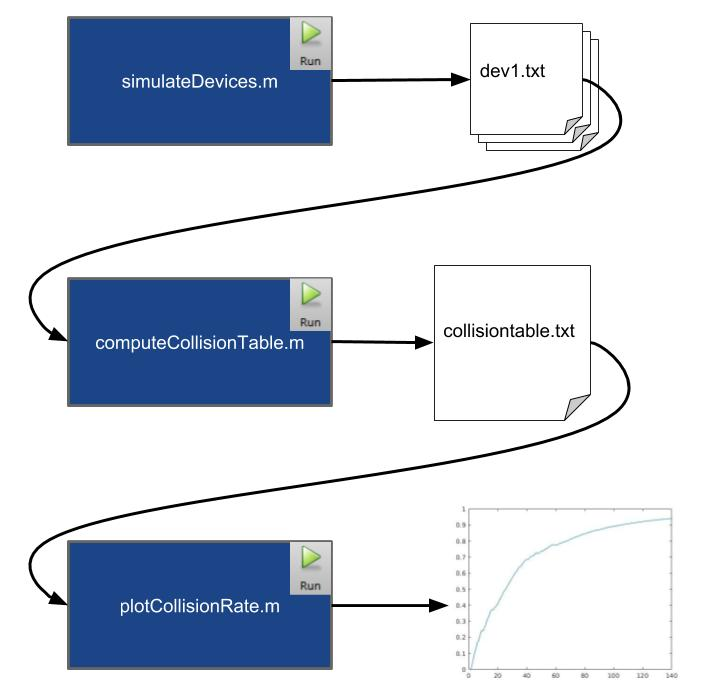
\includegraphics[width=0.8\textwidth]{./figures/simulation}
            \caption{Visualization of the simulation steps}
            \label{fig:simulation}
        \end{figure}

        \begin{enumerate}
                \item Simulate packets sent by the devices:\\
                        Open the project root in Matlab. Open the file:
                        
\begin{verbatim}
+simulator>simulateDevices.m
\end{verbatim}
                        
                        Following simulation parameters can be adjusted:
                        \begin{itemize}
                                \item Simulation duration (duration)
                                \item Bandwidth (bw)
                                \item Spreading Factor (sf)
                                \item Code Rate (cr)
                                \item Date Rate Optimization enabled (de)
                                \item Arrival rate (lambda)
                                \item Minimum payload length (packetDistLower)
                                \item Maximum packet length (packetDistUpper)
                                \item Arrival Distribution (arrivalDist)
                                \item Duty Cycle (dc)
                                \item Header enabled (h)
                                \item Number of simulated devices (numDevices)
                                \item Start address of the first device
                                    (devicedevAddr)
                        \end{itemize}

                        After configuring the device parameters the simulation
                        can be started by executing the current file in Matlab.
                        When the simulation of the packet arrival has finished,
                        the resulting device files are stored in:
                        
\begin{verbatim}
results>simulations>CURRENT_DATE
\end{verbatim}
                        
                        For each device, a file \verb|devN.txt|, has been
                        generated, where N represents the device id. The path
                        where the results are stored can also be adjusted in
                        this file.
            \item Compute the collision table:\\
                        Open the file:

\begin{verbatim}
+plot>+CollisionRate>computeCollisionTable.m
\end{verbatim}
                        
                        Choose the folder with the results of the device
                        simulation described in the former step by adjusting
                        the variable:

\begin{verbatim}
simulationDate = PATH_TO_DEVICE_FILES;
\end{verbatim}
                        
                        Input and output directory can be adjusted in this
                        file. The file can be directly executed in Matlab for
                        the computation of the collisions. After the
                        computation has finished, by default the collision
                        table is stored in:
                        
\begin{verbatim}
results>collisions>SIMULATION_DATE>collisiontable.txt
\end{verbatim}

                        It is a single CSV file containing all packets and the
                        collisions found between packets.
            \item Plot the Collision Rate:\\
                    Open the file:
\begin{verbatim}
+plot>+CollisionRate>plotCollisionRate.m
\end{verbatim}
                    
                    Select the name of the folder containing the collision rate
                    table created in step 2 by adjusting the variable:

\begin{verbatim}
date = SIMULATION_DATE;
\end{verbatim}
                    Execute the file in Matlab. After the collision rate
                    computations have finished, a plot showing the collision
                    rate for the different device numbers opens in a new
                    window.
                    
        \end{enumerate}

\end{appendices}

\newpage
\bibliography{./LoRa.bib}
\bibliographystyle{ieeetr}
\end{document}
